%%%%%%%%%%%%%%%%%%%%%%%%%%%%%%%%%%%%%%%%%
% Memo
% LaTeX Template
% Version 1.0 (30/12/13)
%
% This template has been downloaded from:
% http://www.LaTeXTemplates.com
%
% Original author:
% Rob Oakes (http://www.oak-tree.us) with modifications by:
% Vel (vel@latextemplates.com)
%
% License:
% CC BY-NC-SA 3.0 (http://creativecommons.org/licenses/by-nc-sa/3.0/)
%
%%%%%%%%%%%%%%%%%%%%%%%%%%%%%%%%%%%%%%%%%

\documentclass[letterpaper,11pt]{texMemo} % Set the paper size (letterpaper, a4paper, etc) and font size (10pt, 11pt or 12pt)

\usepackage{fancyhdr}
\usepackage{fancybox}
\usepackage{longtable}
\usepackage{amsmath}
%----------------------------------------------------------------------------------------
%	MEMO INFORMATION
%----------------------------------------------------------------------------------------

\memoto{Luis Andr\'es Valido Fajardo. luis.valido@umcc.cu (53694742)} % Recipient(s)

\memofrom{Josval Díaz Blanco} % Sender(s)

\memosubject{Guía de Aprendizaje para Concursantes ICPC y IOI: Búsqueda Binaria } % Memo subject

\memodate{\today} % Date, set to \today for automatically printing todays date

\logo{
\includegraphics[scale=0.5]{img/icpc}} % Institution logo at the top right of the memo, comment out this line for no logo

%----------------------------------------------------------------------------------------

\begin{document}

%\AddToShipoutPicture{\BackgroundPic}
\maketitle % Print the memo header information
%\tableofcontents

\pagebreak

\pagestyle{fancy}
\fancyhead[LO,CE]{ 
\includegraphics[scale=0.03]{img/logo1}}
\fancyhead[RO,CE]{
\includegraphics[scale=0.1]{img/icpc}}
\fancyfoot[LO,CE]{\textbf{Autor:} Luis Andrés Valido Fajardo \\ \textbf{Email:} luis.valido1989@gmail.com \\ \textbf{Teléfono:} 53694742}
\fancyfoot[RO,CE]{\emph{Existen 10 tipos de personas Las que \\saben binario y LAS QUE NO}}
\fancypagestyle{plain}{\pagestyle{fancy}}



%\lhead{ }
%\rhead{  }

%\fancyfoot[L]{}
%\fancyfoot[R]{\textbf{Autor:} Luis Andrés Valido Fajardo \\ \textbf{Email:} luis.valido@umcc.cu}
%----------------------------------------------------------------------------------------
%	MEMO CONTENT
%----------------------------------------------------------------------------------------


\section{Introducción}
El problema de la subsecuencia creciente más larga (\emph{Longest Increasing Subsequence,LIS}) consiste en encontrar una subsecuencia de una secuencia dada en la que los elementos de la subsecuencia estén ordenados, de menor a mayor, y en la que la subsecuencia sea lo más larga posible. Esta subsecuencia no es necesariamente contigua o única. Por ejemplo, considere la siguiente subsecuencia:

$${0, 8, 4, 12, 2, 10, 6, 14, 1, 9, 5, 13, 3, 11, 7, 15}$$

La subsecuencia creciente más larga es \{0, 2, 6, 9, 11, 15\} de longitud 6; la secuencia de entrada no tiene subsecuencias crecientes de 7 miembros. La subsecuencia creciente más larga en este ejemplo no es única. Por ejemplo, \{0, 4, 6, 9, 11, 15\} y \{0, 4, 6, 9, 13, 15\} son otras subsecuencias crecientes de igual longitud en la misma secuencia de entrada.
\section{Conocimientos previos}
\subsection{Función recursiva}
La recursividad es una técnica de programación que se utiliza para realizar una llamada a una
función desde ella misma, de allí su nombre. Un algoritmo recursivo es un algoritmo que expresa la solución de un problema en términos
de una llamada a sí mismo. La llamada a sí mismo se conoce como llamada recursiva o recurrente.


\subsection{Memorización}
En Informática, el término memorización (del inglés memoization) es una técnica de optimización que se usa principalmente para acelerar los tiempos de cálculo, almacenando los resultados de la llamada a una subrutina en una memoria intermedia o búfer y devolviendo esos mismos valores cuando se llame de nuevo a la subrutina o función con los mismos parámetros de entrada. 


\subsection{Programación Dinámica}
La Programación Dinámica la cual es una técnica que combina la corrección de la búsqueda completa y la eficiencia de los algoritmos golosos.

\subsection{Búsqueda Binaria}
La búsqueda binaria es un algoritmo eficiente para encontrar un elemento en una lista ordenada de elementos. Funciona al dividir repetidamente a la mitad la porción de la lista que podría contener al elemento, hasta reducir las ubicaciones posibles a solo una. 
\section{Desarrollo}
\subsection{Subsecuencia creciente más larga con recursividad}
El problema se puede resolver basándose en la siguiente idea:

Sea L(i) la longitud del LIS que termina en el índice i tal que arr[i] sea el último elemento del LIS. Entonces, L(i) puede escribirse recursivamente como:

$$L(i) = \begin{cases}
	1 + \max(L(j)) &  0 \le j < i \quad y \quad arr[j] < arr[i] \\ 
	
	1 & Si \quad no \quad existe \quad tal \quad j 
\end{cases}$$

Formalmente, la longitud de LIS que termina en el índice $i$ es una unidad mayor que el máximo de longitudes de todos los LIS que terminan en algún índice $j$ tal que $arr[j] < arr[i]$ donde $j < i$.

Veamos la siguiente ejemplo desarrollando el árbol de recursión considerando la siguiente colección $arr[] = \{3, 10, 2, 11\}$ la colección a la cual deseamos cacular el LIS.

% TODO: \usepackage{graphicx} required
\begin{figure}[!h]
	\centering
	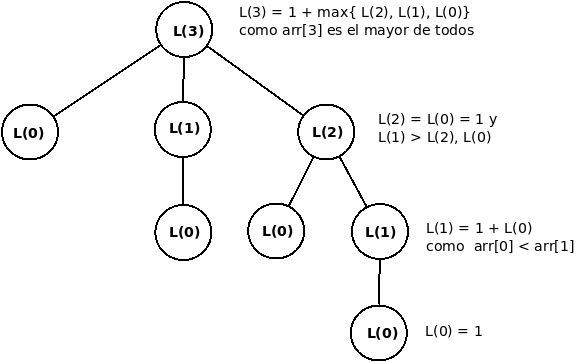
\includegraphics[width=0.7\linewidth]{img/list_recursive_tree}
	\label{fig:listrecursivetree}
\end{figure}


Veamos los pasos a seguir para implementar la idea anterior:

\begin{itemize}
	\item Crea una función recursiva.
	\item Para cada llamada recursiva, itere desde i = 0 hasta la posición actual y haga lo siguiente:
	\begin{itemize}
		\item Encuentre la longitud posible de la subsecuencia creciente más larga que termina en la posición actual si la secuencia anterior terminó en $i$.
		\item Actualice la longitud máxima posible en consecuencia.
	\end{itemize}
	\item Repita esto para todos los índices y encuentre la respuesta.
\end{itemize}


\subsection{Subsecuencia creciente más larga con memorización}
Si se analiza con atención, podemos ver que la solución recursiva anterior también sigue la propiedad de subproblemas superpuestos, es decir, la misma subestructura resuelta una y otra vez en diferentes rutas de llamada recursiva. Podemos evitar esto utilizando el enfoque de memorización.

Podemos ver que cada estado se puede identificar de forma única mediante dos parámetros:

\begin{itemize}
	\item \textbf{Índice actual:} Denota el último índice del LIS.
	\item \textbf{Índice anterior:} Denota el índice final del LIS anterior detrás del cual se concatena el arr[i] es decir el índice actual.
\end{itemize}

La idea es usar una matriz para almacenar los resultados de los diferentes estados que puede generar la recursividad y solo utilizar la recursividad cuando no se haya calculado el valor previamente para ese estado. Esta idea mejora la complejidad temporal pero sacrificando la complejidad espacial.   
\subsection{Subsecuencia creciente más larga con programación dinámica}
Debido a la subestructura óptima y la propiedad de subproblema superpuesta, también podemos utilizar la programación dinámica para resolver el problema. En lugar de memorizar, podemos usar el bucle anidado para implementar la relación recursiva.

El bucle externo se ejecutará desde $i = 1$ hasta $N$ y el bucle interno se ejecutará desde $j = 0$ hasta $i$ y utilizará la relación de recurrencia para resolver el problema.
\subsection{Subsecuencia creciente más larga con búsqueda binaria}
Este enfoque de solución no se apoya en los enfoques anteriores para dar una solución como si sucedió con los enfoques anteriores. Vamos a partir de la idea que en la LIS de una colección puede ser toda la colección en sí, por ejemplo una colección donde todos los elementos son distintos y casualmente están ordenados de forma creciente. Basados en esta idea vamos a construir una colección de depositos $S$ donde en $S[i]$ se almacenará el entero más pequeño que termina una secuencia creciente de longitud $i$. 

La idea principal del enfoque es simular el proceso de encontrar una subsecuencia manteniendo una lista de \emph{depósitos} donde cada depósito representa una subsecuencia válida. Inicialmente, comenzamos con una lista vacía y recorremos los números del vector de entrada de izquierda a derecha.

Para cada número en la colección, realizamos los siguientes pasos:

\begin{itemize}
	\item Si el número es mayor que el último elemento del último depósito (es decir, el elemento más grande en la subsecuencia actual), agregamos el número al final de la lista. Esto indica que hemos encontrado una subsecuencia más larga.
	\item De lo contrario, realizamos una búsqueda binaria en la lista de depósitos para encontrar el elemento más pequeño que sea mayor o igual al número actual. Este paso nos ayuda a mantener la propiedad de aumentar los elementos en los depósitos.
	\item Una vez que encontramos la posición a actualizar, reemplazamos ese elemento con el número actual. Esto mantiene los despositos ordenados y garantiza que tengamos potencial para una subsecuencia más larga en el futuro.
\end{itemize}

Ilustremos esto con la ayuda de un ejemplo. Los siguientes son los pasos seguidos por el algoritmo para un arreglo de enteros $A=\{2, 6, 3, 4, 1, 2, 9, 5, 8\}$:

\begin{enumerate}
	\item Inicializamos la colección de depósito S vacio. $S= \{\}$
	\item Insertando 2  S = \{2\} - Nuevo LIS más grande.
	\item Insertando 6  S = \{2, 6\} - Nuevo LIS más grande.
	\item Insertanto 3  S = \{2, 3\} - Remplaza 6 con 3.
	\item Insertanto 4  S = \{2, 3, 4\} - Nuevo LIS más grande.
	\item Insertanto 1  S = \{1, 3, 4\} - Remplaza 2 con 1
	\item Insertanto 2  S = \{1, 2, 4\} - Remplaza 3 con 2
	\item Insertanto 9  S = \{1, 2, 4, 9\} - Nuevo LIS más grande.
	\item Insertanto 5  S = \{1, 2, 4, 5\} - Remplaza 9 con 5
	\item Insertanto 8  S = \{1, 2, 4, 5, 8\} - Nuevo LIS más grande.
\end{enumerate}

Entonces, la longitud del LIS es 5 (el tamaño de S). Tenga en cuenta que aquí $S[i]$ se define como el entero más pequeño que termina una secuencia creciente de longitud $i$. Por lo tanto, $S$ no representa una secuencia real, pero el tamaño de $S$ representa la longitud LIS.
\section{Implementación}
\subsection{C++}

\subsubsection{Recursividad}
\begin{lstlisting}[language=C++]
int _lis(int arr[], int n, int* max_ref){
   if(n == 1) return 1;
   
   int res, max_ending_here = 1;
   
   for(int i = 1; i < n; i++){
      res = _lis(arr, i, max_ref);
      if(arr[i-1] < arr[n-1] && res+1 > max_ending_here)
         max_ending_here = res + 1;
   }
	
   if (*max_ref < max_ending_here)
      *max_ref = max_ending_here;
	
   return max_ending_here;
}

int lis(int arr[], int n){
   int max = 1;
   _lis(arr, n, &max);
   return max;
}
\end{lstlisting}


\subsubsection{Memorización}
\begin{lstlisting}[language=C++]
int f(int idx, int prev_idx, int n, int a[],vector<vector<int> >& dp){
   if (idx == n) return 0;
   
   if (dp[idx][prev_idx + 1] != -1) return dp[idx][prev_idx + 1];
	
   int notTake = 0 + f(idx + 1, prev_idx, n, a, dp);
   int take = INT_MIN;
   if (prev_idx == -1 || a[idx] > a[prev_idx]) 
      take = 1 + f(idx + 1, idx, n, a, dp);
   
   return dp[idx][prev_idx + 1] = max(take, notTake);
}

int longestSubsequence(int n, int a[]){
   vector<vector<int> > dp(n + 1, vector<int>(n + 1, -1));
   return f(0, -1, n, a, dp);
}
\end{lstlisting}

\subsubsection{Programación Dinámica}
\begin{lstlisting}[language=C++]
int lis(int arr[], int n){
   int lis[n];
   lis[0] = 1;
	
   for (int i=1;i<n;i++){
      lis[i] = 1;
      for (int j = 0; j < i; j++)
         if (arr[i] > arr[j] && lis[i] < lis[j] + 1)
            lis[i] = lis[j] + 1;
   }
   return *max_element(lis, lis + n);
}

\end{lstlisting}

\subsubsection{Búsqueda binaria}
\begin{lstlisting}[language=C++]

int lengthOfLIS(vector<int>& nums){
   int n = nums.size();
   vector<int> ans;
	
   ans.push_back(nums[0]);
	
   for (int i = 1; i < n; i++) {
      if (nums[i] > ans.back()) {
         ans.push_back(nums[i]);
      }
      else {
         int low = lower_bound(ans.begin(), ans.end(),nums[i])-ans.begin();
         ans[low] = nums[i];
      }
   }
   return ans.size();
}
\end{lstlisting}


\subsection{Java}

\subsubsection{Recursividad}
\begin{lstlisting}[language=Java]
class Main {
	
   static int max_ref;
	
   static int _lis(int arr[], int n){
      if (n == 1) return 1;
      
      int res, max_ending_here = 1;
		
      for(int i = 1; i < n; i++){
         res = _lis(arr, i);
         if(arr[i-1] < arr[n-1] && res+1 > max_ending_here)
            max_ending_here = res + 1;
      }
		
      if(max_ref < max_ending_here)
         max_ref = max_ending_here;
		
      return max_ending_here;
    }
	
    static int lis(int arr[], int n){
       max_ref = 1;
       _lis(arr, n);
       return max_ref;
    }
}
\end{lstlisting}

\subsubsection{Memorización}
\begin{lstlisting}[language=Java]
class Main{
   static int f(int idx, int prev_idx, int n, int a[],int[][] dp){
      if (idx == n) return 0;
		
      if (dp[idx][prev_idx + 1] != -1) return dp[idx][prev_idx + 1];
      
      int notTake = 0 + f(idx + 1, prev_idx, n, a, dp);
      int take = Integer.MIN_VALUE;
      if (prev_idx == -1 || a[idx] > a[prev_idx]) 
         take = 1 + f(idx + 1, idx, n, a, dp);
      return dp[idx][prev_idx + 1] = Math.max(take, notTake);
   }
	
   static int lis(int arr[], int n){
      int dp[][] = new int[n + 1][n + 1];
      for (int row[] : dp) Arrays.fill(row, -1);
         return f(0, -1, n, arr, dp);
   }
}
\end{lstlisting}

\subsubsection{Programación Dinámica}
\begin{lstlisting}[language=Java]
class Main {

   static int lis(int arr[], int n){
      int lis[] = new int[n];
      int i, j, max = 0;
		
      for (i = 0; i < n; i++)
         lis[i] = 1;
		
      for (i = 1; i < n; i++)
         for (j = 0; j < i; j++)
            if (arr[i] > arr[j] && lis[i] < lis[j] + 1)
               lis[i] = lis[j] + 1;
		
      for (i = 0; i < n; i++)
         if (max < lis[i])
            max = lis[i];
		
      return max;
   }
}

\end{lstlisting}

\subsubsection{Búsqueda binaria}
\begin{lstlisting}[language=Java]
public class Main {
   static int lengthOfLIS(int[] nums) {
      int n = nums.length;
      List<Integer> ans = new ArrayList<>();
      ans.add(nums[0]);
      
      for (int i = 1; i < n; i++) {
         if (nums[i] > ans.get(ans.size() - 1)) {
            ans.add(nums[i]);
         } else {
		    int low = Collections.binarySearch(ans, nums[i]);
            if (low < 0) {
               low = -(low + 1);
            }
            ans.set(low, nums[i]);
         }
      }
      return ans.size();
   }
}

\end{lstlisting}	
\section{Aplicaciones}
Este es de los problemas de la programación dinámica, uno de los denomindados como clásicos. 

Aunque los problemas de tipo programación dinámica son muy popular con una alta frecuencia de aparición en concursos de programación
recientes, los problemas clásicos de programación dinámica en su forma pura (como el presentado en esta guía) por lo general ya no aparecen en los IOI o ICPC modernos. A pesar de esto es necesario su estudio ya
que nos permite entender la programación dinámica y como poder resolver aquellos problema de programación dinámica clasificados como no-clásicos e incluso nos permite desarrollar nuestras habilidades de programación
dinámica en el proceso.
\section{Complejidad}
Veamos un análisis tanto temporal como espacial de los diferentes enfoques analizados para resolver el problema:

\begin{longtable}{|c|p{5.5cm}|p{5.5cm}|}
	\hline
	& \textbf{Complejidad temporal} & \textbf{Complejidad espacial} \\
	\hline
	\textbf{Recursividad} &  La complejidad temporal de este enfoque recursivo es exponencial O($2^N$) ya que existe un caso de subproblemas superpuestos como se explica en el diagrama de árbol recursivo anterior.  & No se utiliza ningún espacio externo para almacenar valores aparte del espacio de la pila interna por tanto O($1$) \\ \hline
	\textbf{Memorización} & En el peor de los casos se tendría que calcular todos los posibles estados que sería como recorrer todas las posiciones de la matriz por lo que la complejidad es O($N^2$) & Es evidente que el uso de una matriz para almacenar los cálculos de los diferentes estados hace que la complejidad espacial para esta variante es O($N^2$) \\ \hline
	\textbf{Programación Dinámica} & Como la implementación tiene un ciclo anidado dicha implementación tiene una complejidad temporal O($N^2$)  & Como utiliza un arreglo para almacenar el LIS para índice de la colección esta idea tiene una complejidad O($N$)  \\ \hline
	\textbf{Búsqueda Binaria} & Como se recorre todos los elementos y dentro de este recorrido se realiza una busqueda binaria en el peor de los casos la complejidad temporal de esta implementación es O($N\log N$)  &  Como utiliza un arreglo para almacenar el LIS para índice de la colección esta idea tiene una complejidad O($N$)\\ \hline
\end{longtable} 
\section{Ejercicios}
A continuación una lista de ejercicios que se pueden resolver aplicando el abordados en esta guía:

\begin{itemize}
	\item \href{https://cses.fi/problemset/task/1145}{CSES - Increasing Subsequence}
	\item \href{https://dmoj.uclv.edu.cu/problem/glowar} {DMOJ - Calentamiento Global}
\end{itemize}

\end{document}